\chapter{Methodology}
In this chapter I will describe the way I went about this project. I will provide details on my approach regarding the research and actualy development work I did for this project. I would like to start with the data.

\subsection{Data}
I began looking for the appopriate data on Kaggle. Kaggle is an online community of data scientists and machine learning practitioners. Kaggle has repositories of publicly avaliabe data for anyone to download and build models for. The data avaliable on kaggle is oftentimes alread pre cleaned so when you download the data it is ready for use straight away. However in my case I had two major issues when looking on Kaggle for the data.

\begin{itemize}
	\item The data on Kaggle wasn't in the format I wanted.
	\item There wasn't enough data avaliable on the topic of fake news.
\end{itemize}

Nevertheless I managed to download a number of datasets from Kaggle. I loaded the data in a jupyter notebook using the pandas library for python and took stock of the data I had retrived. The columns for the datasets were labelled differently. The datasets also had different approaches to the labelling of the correct classifcation of the data with some datasets using numerical values(1 for true, 3 for semi-true and 5 for fake ) and others using text values(true for true and fake for false). On github I managed to find a datset called all-the-news by Andrew Thompson that conatined approximately 143,000 news articles.


\subsection{Models}
Now that I had my data I needed to decide on how best to select the best model to solve the problem. I had two selection critera.
\begin{itemize}
	\item Highest accuracy
	\item Scalability
\end{itemize}
As I was the sole developer for this project I had to make sure that the models I designed were at the level that one person could do it. State of the art models take years and teams full of experts to create and I was the only person doing this project and I had only a short period of time to do it so I had to make my expectations realistic. The first model I decided to create was the support vector machine(SVM)
\subsubsection{Support Vector Machine(SVM)}
The objective of the support vector machine algorithm is to find a hyperplane in an N-dimensional space(N — the number of features) that distinctly classifies the data points. An example is shown below.

\begin{figure}[h!]
	\caption{An overview of a SVM}
	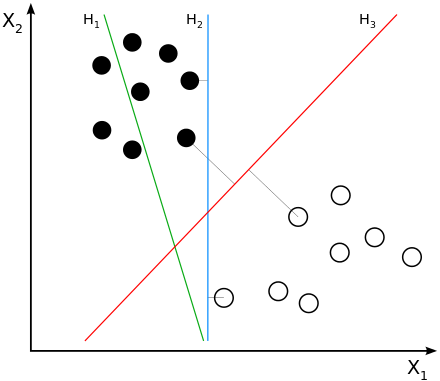
\includegraphics[scale=0.5]{SVM}
\end{figure}

We can see a number of lines drawn in the figure above. A support vector machine aims to find the best line that seperates the two classes. In this case the line H3 does that the best. More formally, a support-vector machine constructs a hyperplane or set of hyperplanes in a high- or infinite-dimensional space, which can be used for classification, regression, or other tasks like outliers detection.

\subsubsection{Long Short Term Memory LSTM}
Long short-term memory (LSTM) is an artificial recurrent neural network (RNN) architecture. An example is shown below

\begin{figure}[h!]
	\caption{An overview of a LSTM cell}
	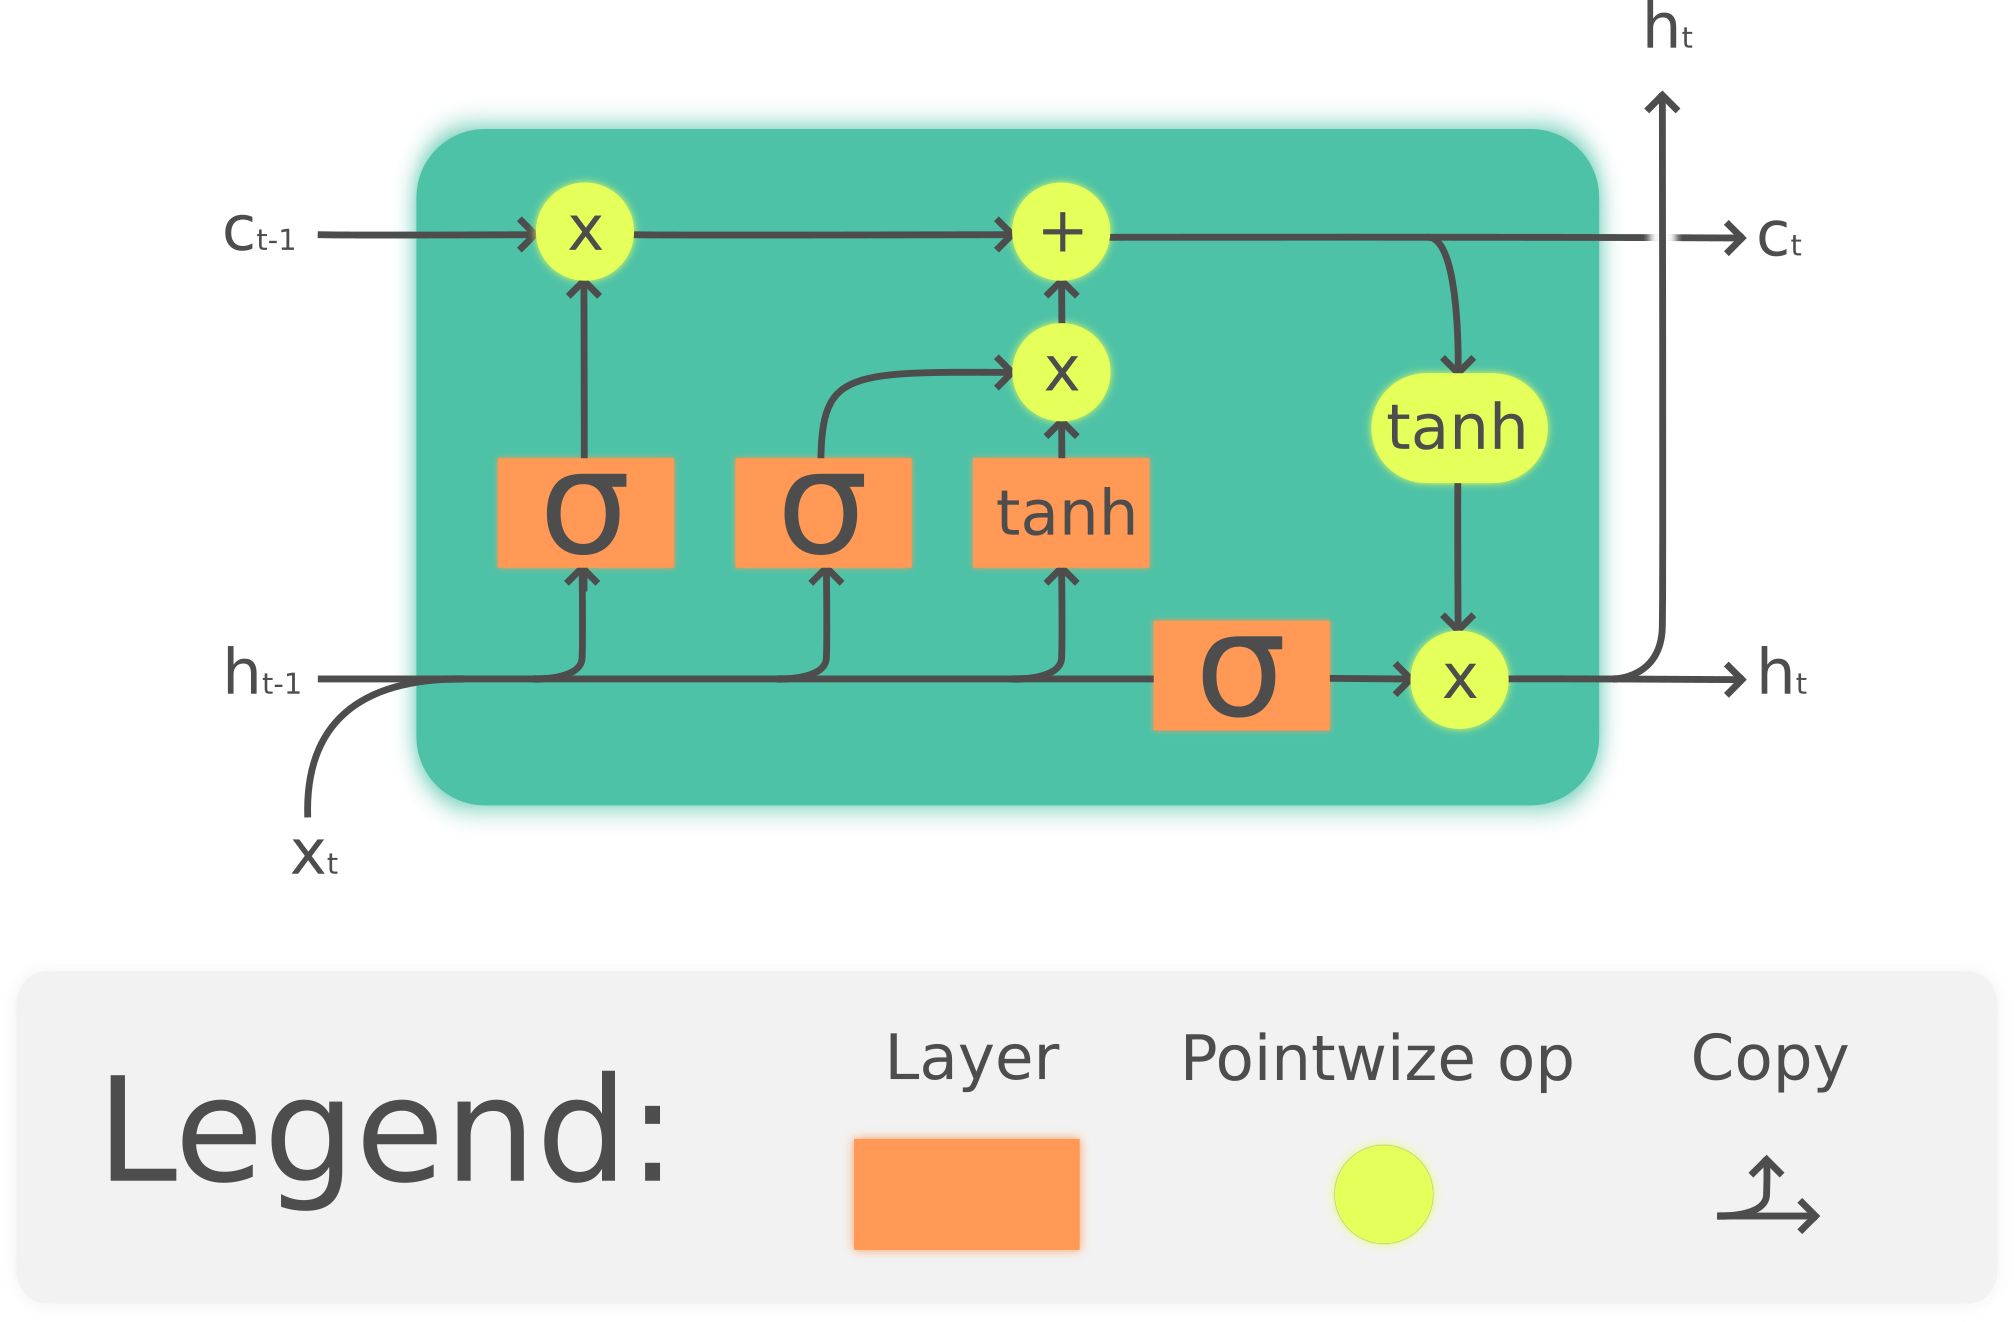
\includegraphics[scale=0.5]{The_LSTM_cell}
\end{figure}


All RNNs have feedback loops in the recurrent layer. This lets them maintain information in 'memory' over time. But, it can be difficult to train standard RNNs to solve problems that require learning long-term temporal dependencies. This is because the gradient of the loss function decays exponentially with time (called the vanishing gradient problem). LSTM networks are a type of RNN that uses special units in addition to standard units. LSTM units include a 'memory cell' that can maintain information in memory for long periods of time. A set of gates is used to control when information enters the memory, when it's output, and when it's forgotten. This architecture lets them learn longer-term dependencies. GRUs are similar to LSTMs, but use a simplified structure. They also use a set of gates to control the flow of information, but they don't use separate memory cells, and they use fewer gates.



\subsection{Testing and Validation}
As I breifly explained in the introduction section of this thesis I used a technique called cross validation to ensure the accuracy of my models. I will now explain cross validation and why I used it in the way that I did.

\subsubsection{Cross Validation}
Cross validation is a technique used in the field of machine learning that aims to combat two major problems

\begin{itemize}
	\item Model Overfitting
	\item Model Underfitting
\end{itemize}
Model overfitting is when a statistical model or machine learning algorithm captures the noise of the data. Intuitively, overfitting occurs when the model or the algorithm fits the data too well.
Overfitting a model result in good accuracy for training data set but poor results on new data sets. Such a model is not of any use in the real world as it is not able to predict outcomes for new cases.

Model underfitting is when a statistical model or machine learning algorithm cannot capture the underlying trend of the data. Intuitively, underfitting occurs when the model or the algorithm does not fit the data well enough. Underfitting is often a result of an excessively simple model. By simple we mean that the missing data is not handled properly, no outlier treatment, removing of irrelevant features or features which do not contribute much to the predictor variable.

\subsection{Deployment}








